% Light Cone Structure in Curved Spacetime
% Demonstrates tipping and deformation of light cones near massive objects
% Foundation for causal structure and event horizons

\begin{figure}[htbp]
\centering
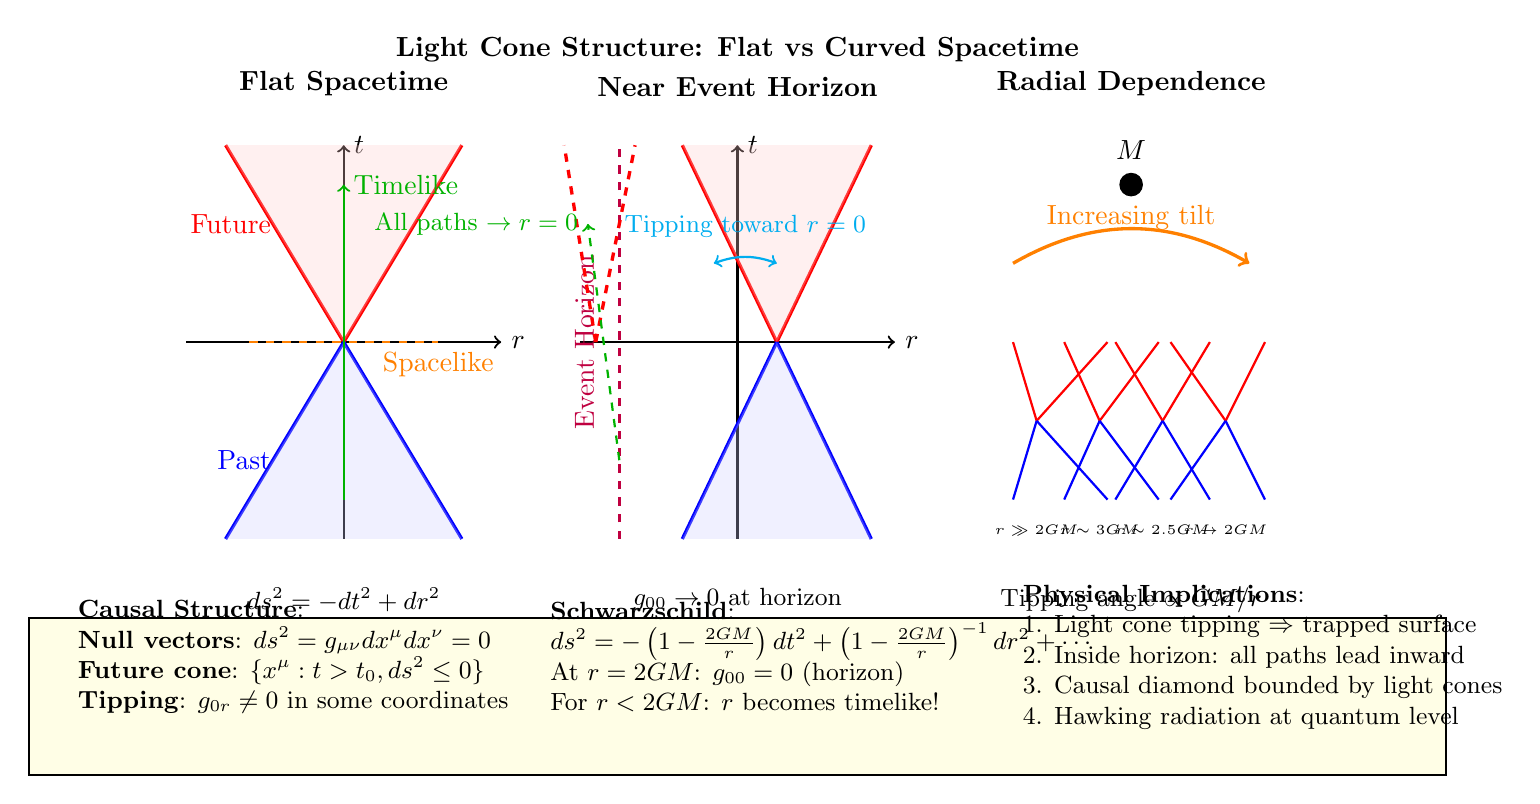
\begin{tikzpicture}[scale=1.0]
    % Title
    \node[anchor=north] at (0,6.5) {\textbf{Light Cone Structure: Flat vs Curved Spacetime}};
    
    % Left: Flat spacetime (Minkowski)
    \begin{scope}[xshift=-5cm]
        \node[above] at (0,5.5) {\textbf{Flat Spacetime}};
        
        % Axes
        \draw[->, thick] (0,0) -- (0,5) node[right] {$t$};
        \draw[->, thick] (-2,2.5) -- (2,2.5) node[right] {$r$};
        
        % Future light cone (symmetric)
        \draw[red, very thick] (0,2.5) -- (-1.5,5);
        \draw[red, very thick] (0,2.5) -- (1.5,5);
        \fill[red!20, opacity=0.3] (0,2.5) -- (-1.5,5) -- (1.5,5) -- cycle;
        
        % Past light cone (symmetric)
        \draw[blue, very thick] (0,2.5) -- (-1.5,0);
        \draw[blue, very thick] (0,2.5) -- (1.5,0);
        \fill[blue!20, opacity=0.3] (0,2.5) -- (-1.5,0) -- (1.5,0) -- cycle;
        
        % Time-like worldline
        \draw[->, green!70!black, thick] (0,0.5) -- (0,4.5);
        \node[green!70!black, right] at (0,4.5) {Timelike};
        
        % Space-like
        \draw[orange, thick, dashed] (-1.2,2.5) -- (1.2,2.5);
        \node[orange, below] at (1.2,2.5) {Spacelike};
        
        % Annotations
        \node[red, left] at (-0.8,4.0) {Future};
        \node[blue, left] at (-0.8,1.0) {Past};
        \node[below, align=center, font=\small] at (0,-0.5) {
            $ds^2 = -dt^2 + dr^2$\\
            Symmetric, unchanging
        };
    \end{scope}
    
    % Center: Schwarzschild near horizon
    \begin{scope}[xshift=0cm]
        \node[above] at (0,5.5) {\textbf{Near Event Horizon}};
        
        % Axes
        \draw[->, thick] (0,0) -- (0,5) node[right] {$t$};
        \draw[->, thick] (-2,2.5) -- (2,2.5) node[right] {$r$};
        
        % Event horizon (vertical dashed line)
        \draw[purple, very thick, dashed] (-1.5,0) -- (-1.5,5);
        \node[purple, above, rotate=90] at (-1.7,2.5) {Event Horizon};
        
        % Tipped light cone at r > 2GM
        \draw[red, very thick] (0.5,2.5) -- (-0.7,5);
        \draw[red, very thick] (0.5,2.5) -- (1.7,5);
        \fill[red!20, opacity=0.3] (0.5,2.5) -- (-0.7,5) -- (1.7,5) -- cycle;
        
        % Past cone (also tipped)
        \draw[blue, very thick] (0.5,2.5) -- (-0.7,0);
        \draw[blue, very thick] (0.5,2.5) -- (1.7,0);
        \fill[blue!20, opacity=0.3] (0.5,2.5) -- (-0.7,0) -- (1.7,0) -- cycle;
        
        % Tipping angle annotation
        \draw[<->, cyan, thick] (0.5,3.5) to[bend right=20] (-0.3,3.5);
        \node[cyan, above, font=\small] at (0.1,3.7) {Tipping toward $r=0$};
        
        % Inside horizon: light cones tip inward
        \draw[red, very thick, dashed] (-1.8,2.5) -- (-2.2,5);
        \draw[red, very thick, dashed] (-1.8,2.5) -- (-1.3,5);
        
        % Worldline forced inward
        \draw[->, green!70!black, thick, dashed] (-1.5,1.0) -- (-1.9,4.0);
        \node[green!70!black, left, font=\small] at (-1.9,4.0) {All paths $\to r=0$};
        
        \node[below, align=center, font=\small] at (0,-0.5) {
            $g_{00} \to 0$ at horizon\\
            Causal structure deformed
        };
    \end{scope}
    
    % Right: Strong field visualization
    \begin{scope}[xshift=5cm]
        \node[above] at (0,5.5) {\textbf{Radial Dependence}};
        
        % Multiple light cones at different radii
        \foreach \x/\tip in {-1.2/0.3, -0.4/0.15, 0.4/0.0, 1.2/-0.1} {
            \draw[red, thick] (\x,1.5) -- (\x-0.6+\tip,2.5);
            \draw[red, thick] (\x,1.5) -- (\x+0.6+\tip,2.5);
            \draw[blue, thick] (\x,1.5) -- (\x-0.6+\tip,0.5);
            \draw[blue, thick] (\x,1.5) -- (\x+0.6+\tip,0.5);
        }
        
        % Radial coordinate labels
        \node[below, font=\tiny] at (-1.2,0.3) {$r \gg 2GM$};
        \node[below, font=\tiny] at (-0.4,0.3) {$r \sim 3GM$};
        \node[below, font=\tiny] at (0.4,0.3) {$r \sim 2.5GM$};
        \node[below, font=\tiny] at (1.2,0.3) {$r \to 2GM$};
        
        % Tipping progression arrow
        \draw[->, orange, very thick] (-1.5,3.5) to[bend left=30] (1.5,3.5);
        \node[orange, above] at (0,3.8) {Increasing tilt};
        
        % Mass source
        \fill[black] (0,4.5) circle (0.15);
        \node[above] at (0,4.7) {$M$};
        
        \node[below, align=center, font=\small] at (0,-0.5) {
            Tipping angle $\propto GM/r$\\
            Causality preserved
        };
    \end{scope}
    
    % Bottom: Mathematical formulation
    \draw[thick, fill=yellow!10] (-9,-1.0) rectangle (9,-3.0);
    
    \node[align=left, font=\small, anchor=west] at (-8.5,-1.5) {
        \textbf{Causal Structure}:\\
        \textbf{Null vectors}: $ds^2 = g_{\mu\nu}dx^\mu dx^\nu = 0$\\
        \textbf{Future cone}: $\{x^\mu : t > t_0, ds^2 \leq 0\}$\\
        \textbf{Tipping}: $g_{0r} \neq 0$ in some coordinates
    };
    
    \node[align=left, font=\small, anchor=west] at (-2.5,-1.5) {
        \textbf{Schwarzschild}:\\
        $ds^2 = -\left(1-\frac{2GM}{r}\right)dt^2 + \left(1-\frac{2GM}{r}\right)^{-1}dr^2 + \cdots$\\
        At $r = 2GM$: $g_{00} = 0$ (horizon)\\
        For $r < 2GM$: $r$ becomes timelike!
    };
    
    \node[align=left, font=\small, anchor=west] at (3.5,-1.5) {
        \textbf{Physical Implications}:\\
        1. Light cone tipping $\Rightarrow$ trapped surface\\
        2. Inside horizon: all paths lead inward\\
        3. Causal diamond bounded by light cones\\
        4. Hawking radiation at quantum level
    };
    
\end{tikzpicture}
\caption{Light cone structure in curved spacetime. Left: flat Minkowski spacetime with symmetric light cones. Center: near Schwarzschild event horizon showing light cone tipping toward $r=0$, with all worldlines forced inward for $r < 2GM$. Right: radial progression showing increasing tilt as $r \to 2GM$. Bottom: mathematical formulation of causal structure and physical implications for black hole horizons.}
\label{fig:lightcone_curved}
\end{figure}
